\subsection{Task 2: Pagerank}
In this experiment, we run pagerank on various size of graph data, 10 in total. The purpose of this design is that we think pagerank is a time consuming operation, and our first try proves our intuition. So we want to test the implementation on incrementally larger dataset, so that we can spot the bottleneck of single machine implementation. 

\begin{center}
\begin{tabular}{| c | c | c |}
    \hline
    Name & Nodes & edges \\ \hline
    Roadnet-ca & 1,965,206 & 5,533,214 \\ \hline
    Roadnet-PA & 1,088,092 & 3,083,796 \\ \hline
    Roadnet-TX & 1,379,917 & 3,843,320 \\ \hline
    com-Amazon & 334,863 & 925,872 \\ \hline
    web-BerkStan & 685,230 & 7,600,595 \\ \hline
    email-Enron & 36,692 & 367,662 \\ \hline
    web-Google & 875,713 & 5,105,039 \\ \hline
    soc-Slashdot0902 & 77,360 & 905,468 \\ \hline
    web-Stanford & 281,903 & 2,312,497 \\ \hline
    wiki-Vote & 7,115 & 103,689 \\ \hline
\end{tabular}
\end{center}

\subsubsection{Detailed Plot}
{\bf Proof of Correctness: } In order to verify the correctness of our implementation, we compare the SQL implementation with a standard implementation with NumPy\footnote{http://www.numpy.org/} on a tiny dataset from "Introduction to Information Retrieval". Table \ref{t2:verify} is the outcome of two different implementaions. We can see that most of the values are the same to one digit of the right of decimal point. The difference after that is due to subtle difference in implmentation, such as max iteration, initilization, etc.

\begin{table}
\begin{center}
\begin{tabular}{| c | c | c | }
    \hline
    Node & SQL & NumPy \\ \hline
    1 & 0.122864 & 0.11799887 \\ \hline
    2 & 0.081234 & 0.08069813 \\ \hline
    3 & 0.263843 & 0.2526222 \\ \hline
    4 & 0.529185 & 0.52647168 \\ \hline
    5 & 0.452971 & 0.45487423 \\ \hline
    6 & 0.081234 & 0.08069813 \\ \hline
    7 & 0.645657 & 0.65203598 \\ \hline
\end{tabular}
\caption{SQL implementaion VS NumPy implementaion}
\label{t2:verify}
\end{center}
\end{table}

Here We use rank-frequency plot to find the underlying patterns in the datasets. 

\paragraph{Roadnet-CA}
The rank-frequency plot(Figure \ref{t2:ca}) of Roadnet-CA is nearly flat, there is not obvious pattern in the plot.
\begin{figure}[!htbf]
\begin{center}
\begin{tabular}{c}
     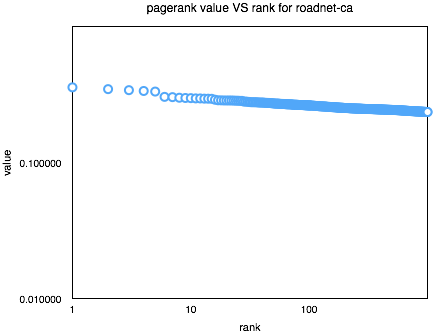
\includegraphics[width=0.6\textwidth]{FIG/t2_ca.png}\\
\end{tabular}
\caption{Rank-frequency plot Roadnet-CA}
\label{t2:ca}
\end{center}
\end{figure}

\paragraph{Roadnet-TX}
The rank-frequency plot(Figure \ref{t2:tx}) of Roadnet-TX is nearly flat, there is not obvious pattern in the plot.
\begin{figure}[!htbf]
\begin{center}
\begin{tabular}{c}
     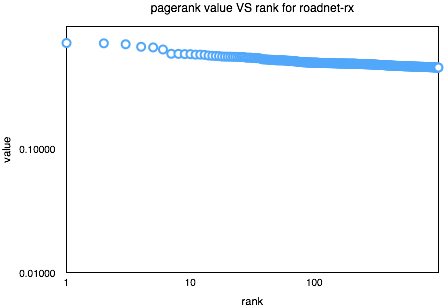
\includegraphics[width=0.6\textwidth]{FIG/t2_tx.png}\\
\end{tabular}
\caption{Rank-frequency plot Roadnet-TX}
\label{t2:tx}
\end{center}
\end{figure}

\paragraph{Roadnet-PA}
The rank-frequency plot(Figure \ref{t2:pa}) of Roadnet-PA is nearly flat, there is not obvious pattern in the plot.
\begin{figure}[!htbf]
\begin{center}
\begin{tabular}{c}
     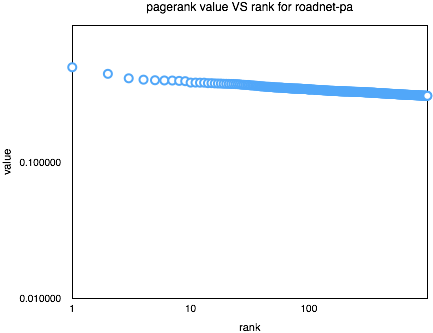
\includegraphics[width=0.6\textwidth]{FIG/t2_pa.png}\\
\end{tabular}
\caption{Rank-frequency plot Roadnet-PA}
\label{t2:pa}
\end{center}
\end{figure}

\paragraph{com-Amazon}
From the plot(Figure \ref{t2:amazon}) we can find that the pagerank distribution follows {\bf power law}, which means that top few nodes has the largest pagerank, while the majority of the node has small pagerank. This matches out intuition in real world data. 
\begin{figure}[!htbf]
\begin{center}
\begin{tabular}{c}
    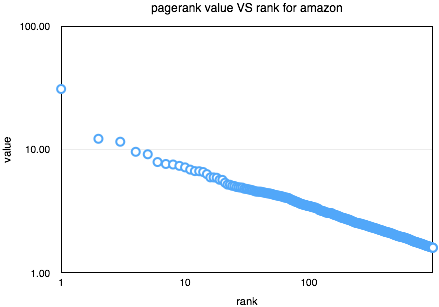
\includegraphics[width=0.6\textwidth]{FIG/t2_amazon.png}
\end{tabular}
\caption{Rank-frequency plot Amazon}
\label{t2:amazon}
\end{center}
\end{figure}

\paragraph{web-BerkStan}
From the plot(Figure \ref{t2:berke}) we can find that the pagerank distribution follows {\bf power law}(exception the first few nodes), which means that top few nodes has the largest pagerank, while the majority of the node has small pagerank. This matches out intuition in real world data. 
\begin{figure}[!htbf]
\begin{center}
\begin{tabular}{c}
    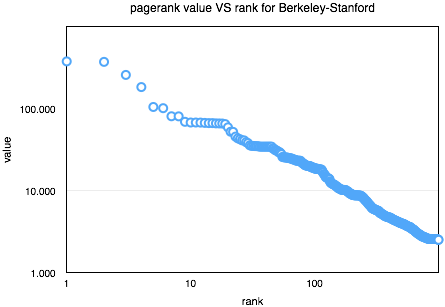
\includegraphics[width=0.6\textwidth]{FIG/t2_berke.png}
\end{tabular}
\caption{Rank-frequency plot BerkeStan}
\label{t2:berke}
\end{center}
\end{figure}

\paragraph{email-Enron}
From the plot(Figure \ref{t2:enron}) we can find that the pagerank distribution follows {\bf power law}(except the first few nodes), which means that top few nodes has the largest pagerank, while the majority of the node has small pagerank. This matches out intuition in real world data. 
\begin{figure}[!htbf]
\begin{center}
\begin{tabular}{c}
    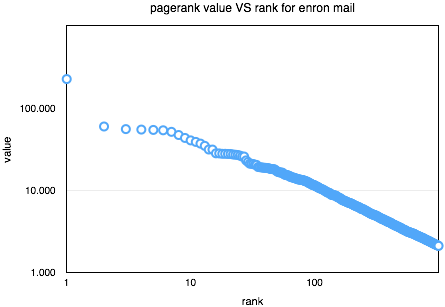
\includegraphics[width=0.6\textwidth]{FIG/t2_enron.png}
\end{tabular}
\caption{Rank-frequency plot Enron mail}
\label{t2:enron}
\end{center}
\end{figure}

\paragraph{web-Google}
From the plot(Figure \ref{t2:google}) we can find that the pagerank distribution follows {\bf power law}, which means that top few nodes has the largest pagerank, while the majority of the node has small pagerank. This matches out intuition in real world data. 
\begin{figure}[!htbf]
\begin{center}
\begin{tabular}{c}
    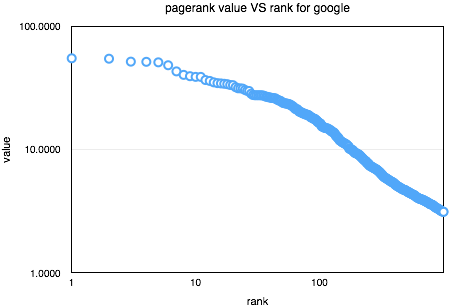
\includegraphics[width=0.6\textwidth]{FIG/t2_google.png}
\end{tabular}
\caption{Rank-frequency plot Google}
\label{t2:google}
\end{center}
\end{figure}

\paragraph{soc-Slashdot0902}
From the plot(Figure \ref{t2:slashdot}) we can find that the pagerank distribution follows {\bf power law}, which means that top few nodes has the largest pagerank, while the majority of the node has small pagerank. This matches out intuition in real world data. 
\begin{figure}[!htbf]
\begin{center}
\begin{tabular}{c}
    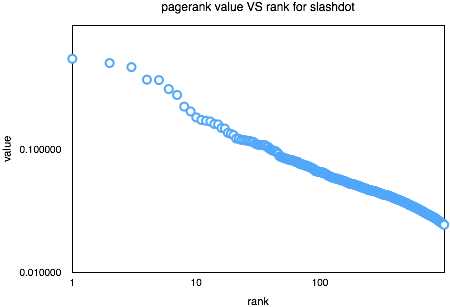
\includegraphics[width=0.6\textwidth]{FIG/t2_slashdot.png}
\end{tabular}
\caption{Rank-frequency plot Slashdot}
\label{t2:slashdot}
\end{center}
\end{figure}

\paragraph{web-Stanford}
From the plot(Figure \ref{t2:stanford}) we can find that the pagerank distribution follows {\bf power law}(except the first few nodes), which means that top few nodes has the largest pagerank, while the majority of the node has small pagerank. This matches out intuition in real world data. 
\begin{figure}[!htbf]
\begin{center}
\begin{tabular}{c}
    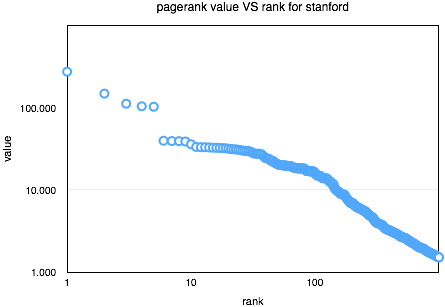
\includegraphics[width=0.6\textwidth]{FIG/t2_stanford.png}
\end{tabular}
\caption{Rank-frequency plot Stanford}
\label{t2:stanford}
\end{center}
\end{figure}

\paragraph{wiki-Vote}
From the plot(Figure \ref{t2:wikivote}) we can find that the pagerank distribution follows {\bf power law}, which means that top few nodes has the largest pagerank, while the majority of the node has small pagerank. This matches out intuition in real world data. 
\begin{figure}[!htbf]
\begin{center}
\begin{tabular}{c}
    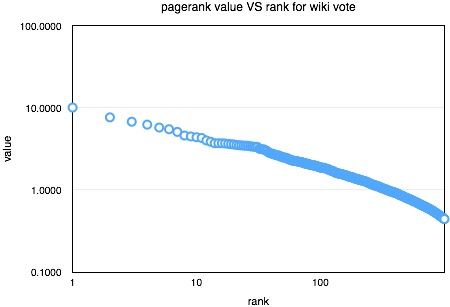
\includegraphics[width=0.6\textwidth]{FIG/t2_wikivote.png}
\end{tabular}
\caption{Rank-frequency plot Wiki-Vite}
\label{t2:wikivote}
\end{center}
\end{figure}


\subsubsection{Observation}
We can observe that in log-log scale, all datasets exhibits linear relationship between rank and frequency. Thus we find another appearance of {\bf power law} in natural graph. An abnormal phenomenon is that the slope of Roadnet datasets is nearly flat. This reflects another aspects of the fundamental property of Roadnet, that all nodes in a roadnet graph are nearly equal to each other, it's a decentralized graph. While in ordinary social network, we always expect to have some important authorities. 




